\section{Problem 4}

\subsection{Question}
\vspace*{10pt}
Rerun A9, Q2 but this time using LIBSVM.  If you have n categories,
you'll have to run it n times.  For example, if you're classifying music
and have the categories:\\
\\
metal, electronic, ambient, folk, hip-hop, pop\\
\\
you'll have to classify things as:\\
\\
metal / not-metal\\
electronic / not-electronic\\
ambient / not-ambient\\
\\
etc.\\
\\
Use the 500 term vectors describing each blog as the features, and
your mannally assigned classifications as the true values.  Use
10-fold cross-validation (as per slide 46, which shows 4-fold
cross-validation) and report the percentage correct for 
each of your categories.\\

\subsection{Answer}
\vspace{2mm}
Using the python script in Listing \ref{listing:gethtml}, 1000 unique URIs were dereferenced and
their raw contents were stored in the {\tt html/raw/} folder as a file with the filename as the
md5-hashed URI. These were then stripped of all html elements and their processed contents were 
stored in the {\tt html/processed/} folder as the same md5-hashed filename. For reference, the URIs were written as the first line of each of their content files.
\vspace{5mm}
\lstinputlisting[language=Python, caption={get\_html.py}, label=listing:gethtml]{q4/get_html.py}
\vspace*{5pt}

\lstinputlisting[language=Python, caption={get\_size.py}, label=listing:getsize]{q4/get_size.py}
\vspace*{5pt}


\textbf{diff} analyzes two files and prints the lines that are different. Essentially, it outputs a set of instructions for how to change one file in order to make it identical to the second file.\\
\\
It does not actually change the files; however, it can optionally generate a script (with the -e option) for the program ed (or ex which can be used to apply the changes.\\
The -e option tells diff to output a script, which can be used by the editing programs ed or ex, that contains a sequence of commands. The commands are a combination of c (change), a (add), and d (delete) which, when executed by the editor, will modify the contents of file1 (the first file specified on the diff command line) so that it matches the contents of file2 (the second file specified).

\lstinputlisting[language=bash, caption={diff command}, label=listing:diff]{q4/diff.sh}


\begin{figure}[h]
\centering
\fbox{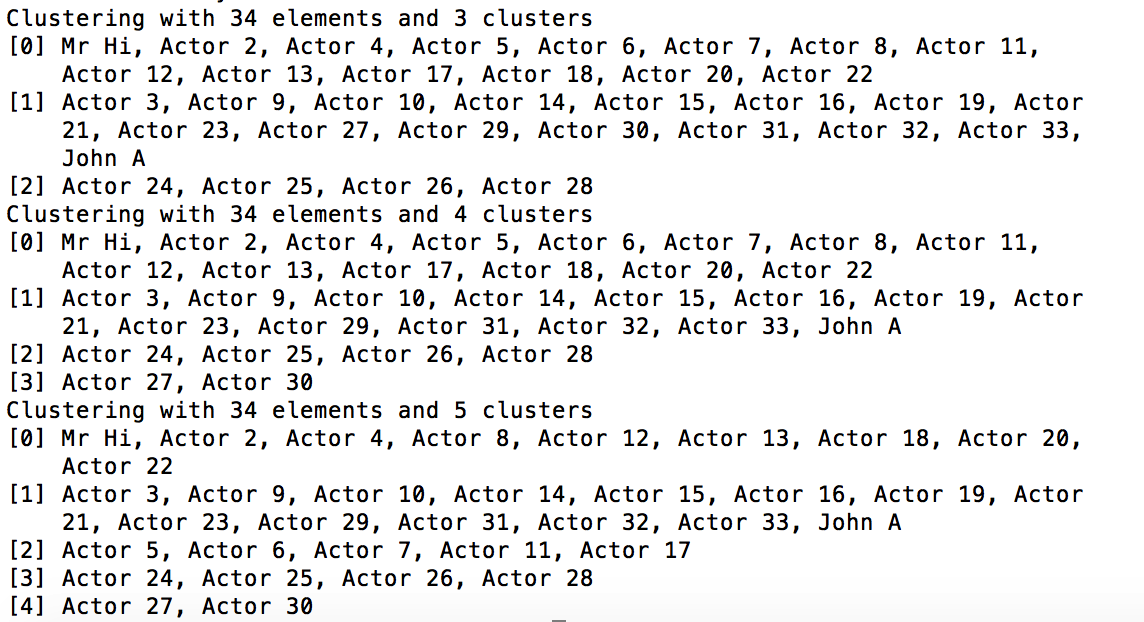
\includegraphics[scale=.75]{q4/fig3.png}}
\caption{Change in Size of Processed Files}
\label{fig:processed}
\end{figure}

\begin{figure}[h]
\centering
\fbox{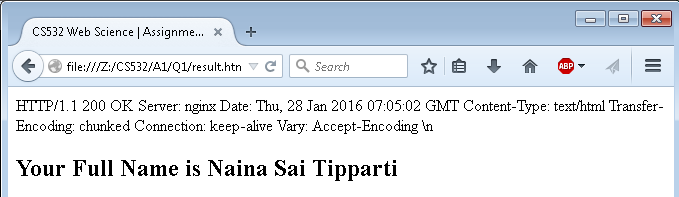
\includegraphics[scale=.65]{q4/fig4.png}}
\caption{Change in Size of Raw Files}
\label{fig:raw}
\end{figure}

